\documentclass{report}

\usepackage{amsmath,amssymb}
\usepackage{graphicx}
\usepackage{enumitem}
\usepackage[total={6in,8in}]{geometry}
\usepackage{multicol}

\newcommand{\sol}{\textbf{Solution:}}
\newcommand{\proof}{\textbf{Proof:}}
\newcommand\perm[2][^n]{\prescript{#1\mkern-2.5mu}{}P_{#2}}
\newcommand\permtwo[2][^n]{{}_{#1}P_{#2}}
\newcommand\comb[2][^n]{{}_{#1}C_{#2}}
\newcommand\combtwo[2][^n]{\prescript{#1\mkern-2.5mu}{}C_{#2}}

\allowdisplaybreaks
\begin{document}
\begin{enumerate}[leftmargin=*]
    \item Given that $f: x \rightarrow 3 x+4$, find

          \begin{enumerate}
              \item $f^{-1}(x)$,

                    \sol{}

                    Let $y = f^{-1}(x)$, then $f(y) = x$.
                    \begin{align*}
                        x         & = 3y + 4        \\
                        3y        & = x - 4         \\
                        y         & = \frac{x-4}{3} \\
                        f^{-1}(x) & = \frac{x-4}{3}
                    \end{align*}

              \item $f^{-1}(5)$,

                    \sol{}
                    \begin{align*}
                        f^{-1}(5) & = \frac{5-4}{3} \\
                                  & = \frac{1}{3}
                    \end{align*}

              \item the value of $x$ such that $f(x)=7$.

                    \sol{}
                    \begin{align*}
                        f(x) & = 7 \\
                        3x+4 & = 7 \\
                        3x   & = 3 \\
                        x    & = 1
                    \end{align*}
          \end{enumerate}

    \item Given that the function $f: x \rightarrow x-4$ and $g: x \rightarrow x^2-3
              x+5$, find
          \begin{enumerate}
              \item $f g(2)$,

                    \sol{}
                    \begin{align*}
                        f g(2) & = f(g(2))       \\
                               & = f(2^2-3(2)+5) \\
                               & = f(4-6+5)      \\
                               & = f(3)          \\
                               & = 3-4           \\
                               & = -1
                    \end{align*}

                    \newpage
              \item the values of $x$ when $f g(x)=5$.

                    \sol{}
                    \begin{align*}
                        f g(x)      & = 5               \\
                        f(x^2-3x+5) & = 5               \\
                        x^2-3x+5-4  & = 5               \\
                        x^2-3x-4    & = 0               \\
                        (x-4)(x+1)  & = 0               \\
                        x = -1      & \text{ or } x = 4
                    \end{align*}
          \end{enumerate}

    \item \begin{enumerate}
              \item Form a quadratic equation which has the roots 4 and -3.

                    \sol{}

                    \begin{align*}
                        (x-4)(x+3)   & = 0 \\
                        x^2+3x-4x-12 & = 0 \\
                        x^2-x-12     & = 0
                    \end{align*}

              \item It is given that $x^2-4 a x+3 b=0$ has two equal real roots. Express $a$ in
                    terms of $b$.

                    \sol{}
                    \begin{align*}
                        b^2-4ac   & = 0                                                   \\
                        16a^2-12b & = 0                                                   \\
                        16a^2     & = 12b                                                 \\
                        a^2       & = \frac{12b}{16}                                      \\
                                  & = \frac{3b}{4}                                        \\
                        a         & = \pm \sqrt{\frac{3b}{4}} = \pm \dfrac{1}{2}\sqrt{3b}
                    \end{align*}
          \end{enumerate}

    \item \begin{enumerate}
              \item Solve the equation:
                    \[3^{x-5}=35^{x-3}\]

                    \sol{}
                    \begin{align*}
                        3^{x-5}            & =35^{x-3}                                  \\
                        \log 3^{x-5}       & =\log 35^{x-3}                             \\
                        (x-5) \log 3       & =(x-3) \log 35                             \\
                        x \log 3-5\log 3   & =x \log 35-3\log 35                        \\
                        x \log 3-x \log 35 & =5\log 3 - 3\log 35                        \\
                        x(\log 3-\log 35)  & =5\log 3 - 3\log 35                        \\
                        x                  & =\frac{5\log 3 - 3\log 35}{\log 3-\log 35} \\
                                           & \approx 2.106
                    \end{align*}

                    \newpage
              \item Solve $\ln (5 x-3)=7$.

                    \sol{}
                    \begin{align*}
                        e^{\ln (5 x-3)} & = e^7             \\
                        5 x-3           & = e^7             \\
                        5 x             & = e^7+3           \\
                        x               & = \frac{e^7+3}{5} \\
                                        & \approx 219.93
                    \end{align*}
          \end{enumerate}

    \item \begin{enumerate}
              \item Find the sum of the first 25 terms of an arithmetic progression $3,5,7, \ldots$

                    \sol{}

                    From the progression, we know that $a=3$, $d=5-3=2$, and $n=25$.
                    \begin{align*}
                        S_{n} & = \dfrac{n}{2}\left[2a + (n-1)d\right]     \\
                              & = \dfrac{25}{2}\left[2(3) + (25-1)2\right] \\
                              & = 675
                    \end{align*}

              \item It is given that the sum of the first ten terms of an arithmetic progression is
                    430 and the sum of the next ten terms is 630. Find the first term and the
                    common difference of the progression.

                    \sol{}

                    Let $a$ be the first term and $d$ be the common difference. Then
                    \begin{align*}
                        S_{10}                                       & = \dfrac{10}{2}\left[2a + (10-1)d\right] = 430 \\
                                                                     & = 5(2a+9d) = 430                               \\
                        2a+9d                                        & = 86\ \cdots\ (1)                              \\
                        S_{20} - S_{10}                              & = 630                                          \\
                        \dfrac{20}{2}\left[2a + (20-1)d\right] - 430 & = 630                                          \\
                        10(2a+19d)                                   & = 1060                                         \\
                        2a+19d                                       & = 106\ \cdots\ (2)
                    \end{align*}
                    \begin{align*}
                        (2) - (1) \Rightarrow 10d & = 20 \\
                        d                         & = 2  \\
                        2a+9(2)                   & = 86 \\
                        2a+18                     & = 86 \\
                        2a                        & = 68 \\
                        a                         & = 34
                    \end{align*}
                    $\therefore$ the first term is 34 and the common difference is 2.
          \end{enumerate}

          \newpage
    \item \begin{enumerate}
              \item Prove that $\dfrac{\cos (A+B)}{\sin A \cos B}=\cot A-\tan B$.

                    \proof{}
                    \begin{align*}
                        \text{L.H.S.} & = \dfrac{\cos (A+B)}{\sin A \cos B}                                           \\
                                      & = \dfrac{\cos A \cos B - \sin A \sin B}{\sin A \cos B}                        \\
                                      & = \dfrac{\cos A \cos B}{\sin A \cos B} - \dfrac{\sin A \sin B}{\sin A \cos B} \\
                                      & = \dfrac{\cos A}{\sin A} - \dfrac{\sin B}{\cos B}                             \\
                                      & = \cot A - \tan B                                                             \\
                                      & = \text{R.H.S.}
                    \end{align*}

              \item Solve the equation $2\cos{2x} = 1 - \cos x$ for $0^{\circ} \leq x \leq
                        360^{\circ}$.

                    \sol{}
                    \begin{align*}
                        2\cos{2x}                           & = 1 - \cos x                 \\
                        2(2\cos^2 x-1)                      & = 1 - \cos x                 \\
                        4\cos^2 x-2                         & = 1 - \cos x                 \\
                        4\cos^2 x+\cos x-3                  & = 0                          \\
                        (4\cos x-3)(\cos x+1)               & = 0                          \\
                        \cos x                = \frac{3}{4} & \text{ or } \cos x = -1      \\
                        x = 41.41^{\circ},\                 & 180^{\circ},\ 318.59^{\circ}
                    \end{align*}

          \end{enumerate}

    \item Diagram 1 shows a straight line $AB$. It is given that $M$ is the midpoint of
          the straight line $AB$ and the coordinates of points $A$, $M$, and $B$ are $(h,
              2)$, $(3, 4)$, and $(8, k)$ respectively.
          \begin{center}
              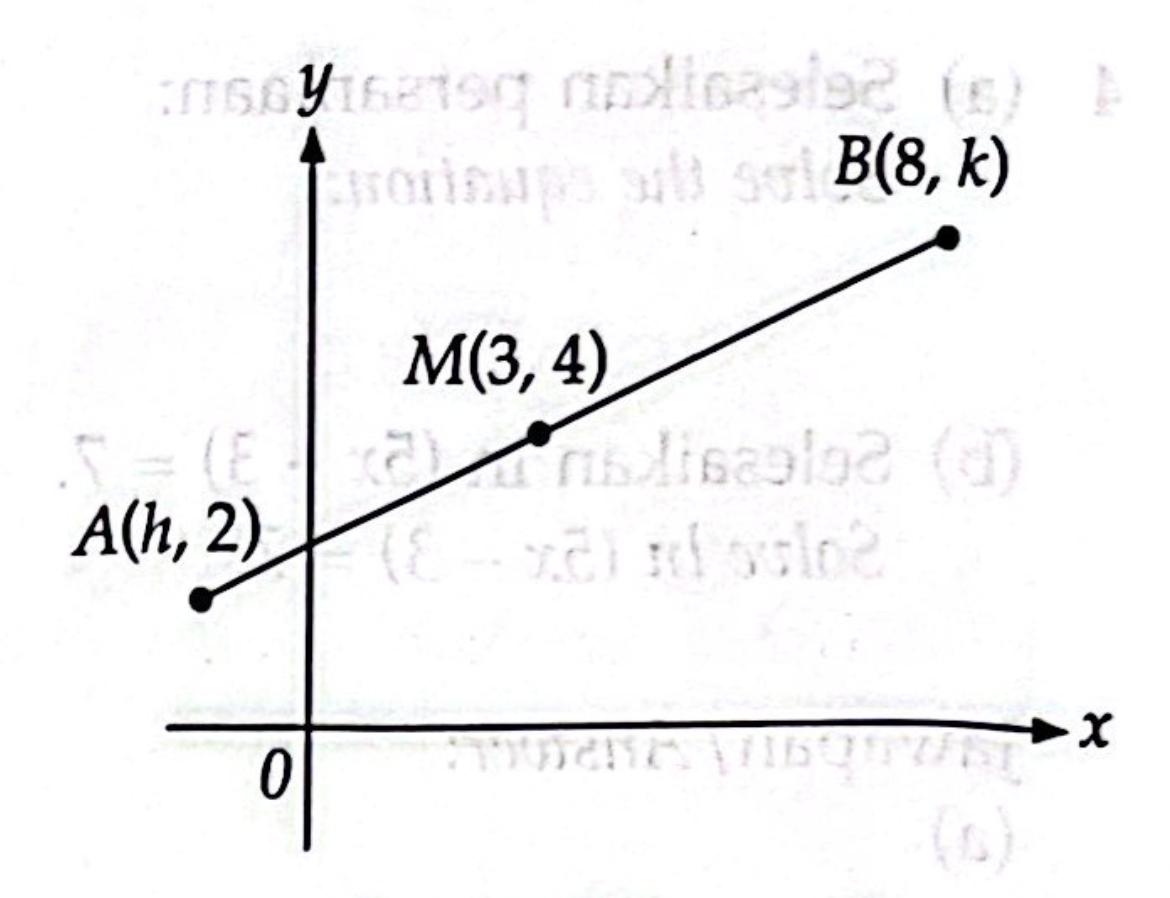
\includegraphics[scale=0.1]{assets/7.png}
          \end{center}
          Find:
          \begin{enumerate}
              \item the value of $h$ and $k$,

                    \sol{}
                    \vspace{-0.8cm}
                    \begin{multicols}{2}
                        \begin{align*}
                            \dfrac{8 + h}{2} & = 3  \\
                            8 + h            & = 6  \\
                            h                & = -2
                        \end{align*}

                        \begin{align*}
                            \dfrac{k+2}{2} & = 4 \\
                            k+2            & = 8 \\
                            k              & = 6
                        \end{align*}
                    \end{multicols}

              \item the gradient of the straight line $AB$, and

                    \sol{}
                    \begin{align*}
                        m & = \dfrac{6 -4}{8 - 3} \\
                          & = \dfrac{2}{5}
                    \end{align*}

              \item the equation fo the perpendicular bisector of $AB$.

                    \sol{}
                    \begin{align*}
                        \text{Gradient of the perpendicular bisector} & = -\dfrac{1}{m}            \\
                                                                      & = -\dfrac{1}{\dfrac{2}{5}} \\
                                                                      & = -\dfrac{5}{2}
                    \end{align*}
                    Therefore the equation of the perpendicular bisector is
                    \begin{align*}
                        y-4    & = -\dfrac{5}{2}(x-3)             \\
                        2y - 8 & = -5x + 15                       \\
                        2y     & = -5x + 23                       \\
                        y      & = -\dfrac{5}{2}x + \dfrac{23}{2}
                    \end{align*}
          \end{enumerate}

    \item It is given that $y = 2x^2 - 4x + 6$. When $x = 2$, there is a small change of
          $x$ of $3\%$. Find the corresponding percentage of change in $y$.

          \sol{}
          \begin{align*}
              y                          & = 2x^2 - 4x + 6                 \\
              \dfrac{dy}{dx}             & = 4x - 4                        \\
              \dfrac{\delta y}{\delta x} & \approx \dfrac{dy}{dx}          \\
              \delta y                   & \approx \dfrac{dy}{dx} \delta x
          \end{align*}
          When $x = 2$, $\delta x = 3\%x = 0.03x = 0.06$, $\dfrac{dy}{dx} = 4(2) - 4 = 4$. Therefore
          \begin{align*}
              \delta y & \approx 4 \times 0.06 \\
                       & = 0.24
          \end{align*}
          Therefore the percentage change in $y$ is
          \begin{align*}
              \dfrac{\delta y}{y} \times 100 & = \dfrac{0.24}{2(2)^2 - 4(2) + 6} \times 100 \\
                                             & = \dfrac{0.24}{6} \times 100                 \\
                                             & = 4\%
          \end{align*}

    \item It is given that the position vector of town $A$ is $-8\vec{\imath} +
              8\vec{\jmath}$ and the position vector of town $B$ is $8\vec{\imath} -
              9\vec{\jmath}$. THe towns $A$, $B$, and $C$ are collinear such that the
          distance between town $A$ and town $C$ is twice the distance between town $A$
          and town $B$. THe distance between the towns is in km. Find
          \begin{enumerate}
              \item $\overrightarrow{AB}$

                    \sol{}
                    \begin{align*}
                        \overrightarrow{AB} & = \overrightarrow{AO} + \overrightarrow{OB}                        \\
                                            & = 8\vec{\imath} - 9\vec{\jmath} - (-8\vec{\imath} + 8\vec{\jmath}) \\
                                            & = 16\vec{\imath} - 17\vec{\jmath}
                    \end{align*}

              \item the distance, in km, between town $A$ and town $B$.

                    \sol{}
                    \begin{align*}
                        \text{Distance} & = |AB|                    \\
                                        & = \sqrt{(16)^2 + (-17)^2} \\
                                        & = \sqrt{256 + 289}        \\
                                        & = \sqrt{545}              \\
                                        & \approx 23.52 \text{ km}
                    \end{align*}

              \item $\overrightarrow{OC}$

                    \sol{}
                    \begin{align*}
                        \overrightarrow{AC} & = 2\overrightarrow{AB}                                               \\
                                            & = 2(16\vec{\imath} - 17\vec{\jmath})                                 \\
                                            & = 32\vec{\imath} - 34\vec{\jmath}                                    \\
                        \overrightarrow{AC} & = \overrightarrow{OC} - \overrightarrow{OA}                          \\
                        \overrightarrow{OC} & = \overrightarrow{AC} + \overrightarrow{OA}                          \\
                                            & = 32\vec{\imath} - 34\vec{\jmath} + (-8\vec{\imath} + 8\vec{\jmath}) \\
                                            & = 24\vec{\imath} - 26\vec{\jmath}
                    \end{align*}
          \end{enumerate}

          \newpage
    \item Given that $\dfrac{d}{dx}\left(\dfrac{dy}{dx}\right) = 6x - 8$ adn the gradient
          function of the curve is 2 when $x = 1$. Find the equation of the curve which
          passes through the point $(2, 3)$.

          \sol{}
          \begin{align*}
              \dfrac{d}{dx}\left(\dfrac{dy}{dx}\right) & = 6x - 8           \\
              \dfrac{dy}{dx}                           & = \int (6x - 8) dx \\
                                                       & = 3x^2 - 8x + c
          \end{align*}
          When $x=1$, $\dfrac{dy}{dx} = 2$.
          \begin{align*}
              2 & = 3(1)^2 - 8(1) + c \\
              c & = 2 - 3 + 8         \\
                & = 7
          \end{align*}
          Therefore $\dfrac{dy}{dx} = 3x^2 - 8x + 7$.
          \begin{align*}
              \dfrac{dy}{dx} & = 3x^2 - 8x + 7           \\
              \int dy        & = \int (3x^2 - 8x + 7) dx \\
              y              & = x^3 - 4x^2 + 7x + c
          \end{align*}
          When $x = 2$, $y = 3$.
          \begin{align*}
              3 & = 2^3 - 4(2)^2 + 7(2) + c \\
              c & = 3 - 8 + 16 - 14         \\
                & = -3
          \end{align*}
          Therefore the equation of the curve is $y = x^3 - 4x^2 + 7x - 3$.

    \item \begin{enumerate}
              \item Five workers, $A$, $B$, $C$, $D$, and $E$, are to be arranged in a row. Find
                    the number of possible arrangement if
                    \begin{enumerate}[]
                        \item there are no conditions,

                              \sol{}

                              The number of possible arrangements is $\permtwo[5]{5} = 5! = 120$.

                        \item the workers $A$ and $B$ are always together.

                              \sol{}

                              Since $A$ and $B$ are always together, we can treat them as one entity.
                              Therefore the number of possible arrangements is $\permtwo[4]{4} \times 2! =
                                  48$.

                    \end{enumerate}
                    \newpage
              \item A class monitor wants to divide 10 students into three groups such that the
                    groups consist of 2 members, 3 members and 5 members. Find the number of
                    different ways to divide all the students.

                    \sol{}

                    First, choose 2 students from 10, we have $\comb[10]{2}$. Then choose 3
                    students from remaining 8, we have $\comb[8]{3}$. The remaining 5 students form
                    the last group. Therefore the number of different ways to divide all the
                    students is
                    \begin{align*}
                        \comb[10]{2} \times \comb[8]{3} & = 45 \times 56 \\
                                                        & = 2520
                    \end{align*}
          \end{enumerate}

    \item During winter, the probability that it will snow on a particular day is $0.55$.
          Find the probability that in a particular week, it will snow
          \begin{enumerate}
              \item exactly 3 days,

                    \sol{}

                    The probability that it will snow on a particular day is $0.55$. Therefore the
                    probability that it will not snow on a particular day is $1 - 0.55 = 0.45$. The
                    probability that it will snow exactly 3 days in a week is
                    \begin{align*}
                        \comb[7]{3} (0.55)^3 (0.45)^4 & = 0.2388
                    \end{align*}

              \item more than 2 days.

                    \sol{}
                    \begin{align*}
                        P(\text{more than 2 days}) & = 1 - P(\text{less than or equal to 2 days})                                                               \\
                                                   & = 1 - \left[\comb[7]{0}(0.55)^0(0.45)^7 + \comb[7]{1}(0.55)^1(0.45)^6 + \comb[7]{2}(0.55)^2(0.45)^5\right] \\
                                                   & = 1 - \left[0.003736 + 0.031969 + 0.117221\right]                                                          \\
                                                   & = 1 - 0.152926                                                                                             \\
                                                   & = 0.8471
                    \end{align*}

              \item Given that a discrete random variable $X \sim B(160, 0.3)$, find the mean and
                    the variance.

                    \sol{}
                    \begin{align*}
                        \mu      & = np = 160 \times 0.3 = 48               \\
                        \sigma^2 & = npq = 160 \times 0.3 \times 0.7 = 33.6
                    \end{align*}
          \end{enumerate}

          \newpage
    \item Diagram 2 shows the road in a residential area. It is given that $OP =
              \vec{u}$, $OQ = \vec{v}$, $3OR = 2OP$ and $PQ = 2PS$. Building $R$ is situated
          in road $OP$, building $S$ is situated in road $PQ$ and building $T$ is
          situated at the intersection of the roads $QR$ and $OS$.
          \begin{center}
              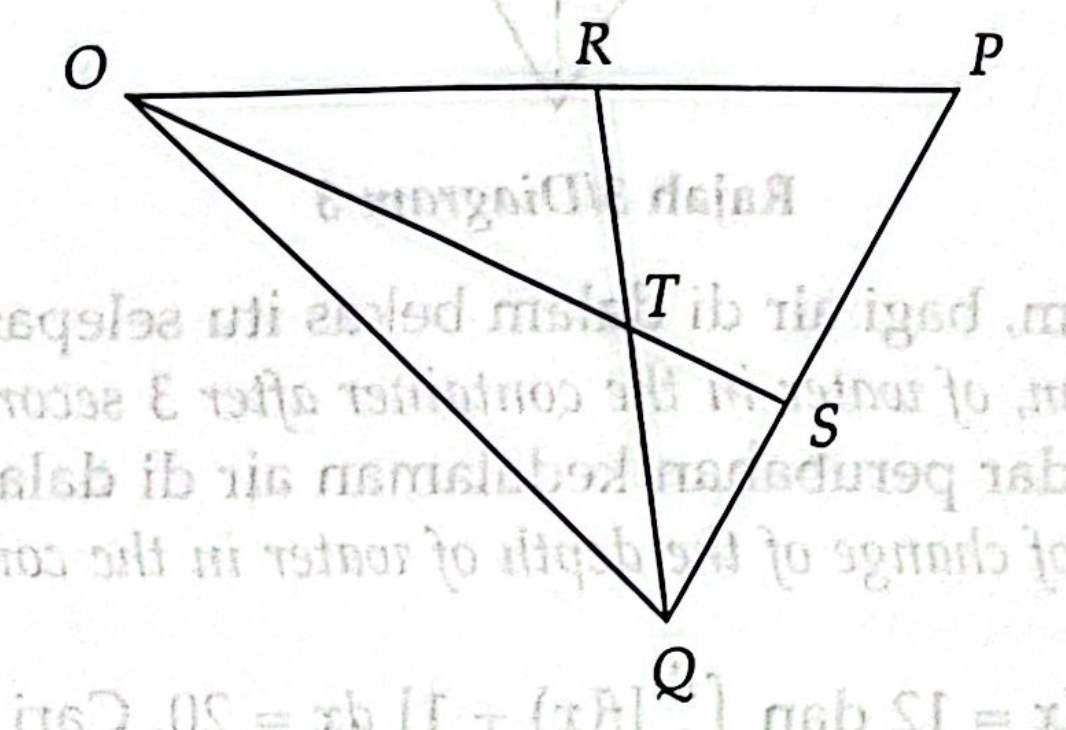
\includegraphics[scale=0.2]{assets/13.png}
          \end{center}

          \begin{enumerate}
              \item Express the following vectors in terms of $\vec{u}$ and $\vec{v}$.

                    \begin{enumerate}
                        \item $\overrightarrow{QR}$

                              \sol{}
                              \begin{align*}
                                  \overrightarrow{QR} & = \overrightarrow{OR} - \overrightarrow{OQ}             \\
                                                      & = \dfrac{2}{3}\overrightarrow{OP} - \overrightarrow{OQ} \\
                                                      & = \dfrac{2}{3}\vec{u} - \vec{v}
                              \end{align*}

                        \item $\overrightarrow{OS}$

                              \sol{}
                              \begin{align*}
                                  \overrightarrow{OS} & = \overrightarrow{OQ} + \overrightarrow{QS}                         \\
                                                      & = \vec{v} - \dfrac{1}{2}\overrightarrow{PQ}                         \\
                                                      & = \vec{v} - \dfrac{1}{2}(\overrightarrow{PO} + \overrightarrow{OQ}) \\
                                                      & = \vec{v} - \dfrac{1}{2}(-\vec{u} + \vec{v})                        \\
                                                      & = \dfrac{1}{2}\vec{v} + \dfrac{1}{2}\vec{u}                         \\
                                                      & = \dfrac{1}{2}(\vec{u} + \vec{v})
                              \end{align*}
                    \end{enumerate}

              \item It is given that $OT = mOS$ and $QT = nQR$, where $m$ and $n$ are constants.
                    Express $\overrightarrow{OT}$ in terms of
                    \begin{enumerate}
                        \item $m$, $\vec{u}$, and $\vec{v}$,

                              \sol{}
                              \begin{align*}
                                  \overrightarrow{OT} & = m\overrightarrow{OS}                          \\
                                                      & = m\left[\dfrac{1}{2}(\vec{u} + \vec{v})\right] \\
                                                      & = \dfrac{m}{2}(\vec{u} + \vec{v})
                              \end{align*}

                        \item $n$, $\vec{u}$, and $\vec{v}$.

                              \sol{}
                              \begin{align*}
                                  \overrightarrow{OT} & = \overrightarrow{OQ} + \overrightarrow{QT}             \\
                                                      & = \vec{v} + n\overrightarrow{QR}                        \\
                                                      & = \vec{v} + n\left[\dfrac{2}{3}\vec{u} - \vec{v}\right] \\
                                                      & = \vec{v} + \dfrac{2}{3}n\vec{u} - n\vec{v}             \\
                                                      & = \dfrac{2}{3}n\vec{u} + (1-n)\vec{v}
                              \end{align*}
                    \end{enumerate}

              \item Hence, find the value of $m$ and $n$.

                    \sol{}
                    \begin{align*}
                        \dfrac{m}{2}(\vec{u} + \vec{v}) & = \dfrac{2}{3}n\vec{u} + (1-n)\vec{v} \\
                        3m\vec{u} + 3m\vec{v}           & = 4n\vec{u} + 6(1-n)\vec{v}
                    \end{align*}
                    Equating the coefficients of $\vec{u}$ and $\vec{v}$, we have
                    \begin{align*}
                        3m  & = 4n           \\
                        3m  & = 6 - 6n       \\
                        4n  & = 6 - 6n       \\
                        10n & = 6            \\
                        n   & = \dfrac{3}{5} \\
                        m   & = \dfrac{4}{5}
                    \end{align*}
          \end{enumerate}

          \newpage
    \item Diagram 4 shows a conical container with a radius of $r$ cm and a height of $h$
          cm. Water is poured into the container at a constant rate of $20$
          cm$^3$s$^{-1}$. it is given that the height of the container is three times the
          radius.
          \begin{center}
              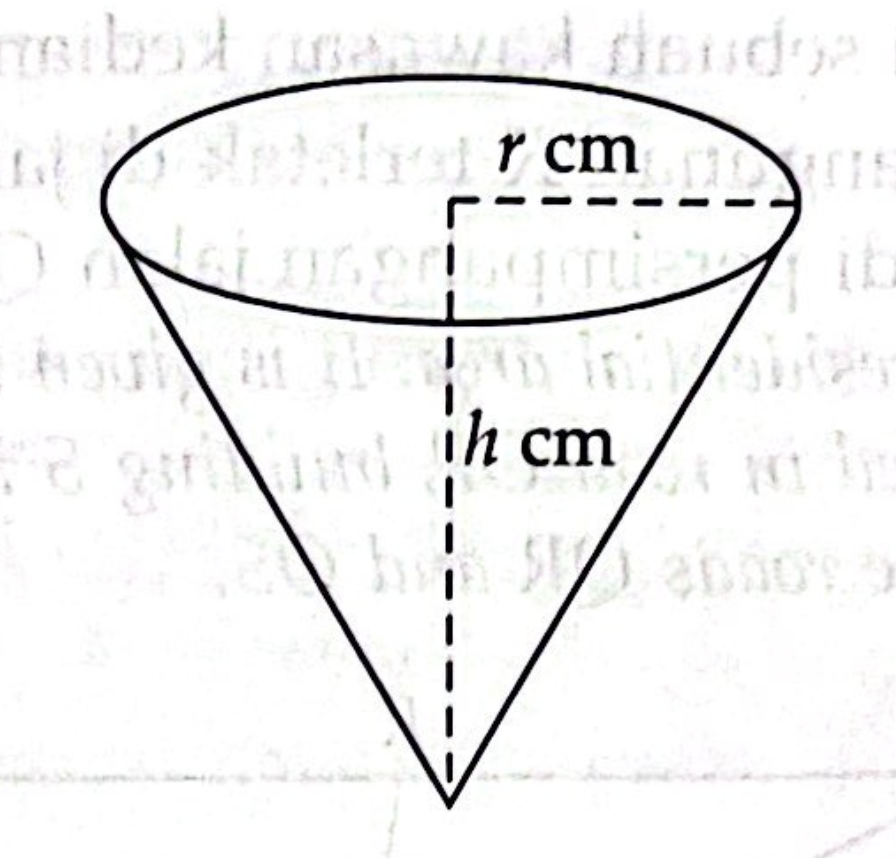
\includegraphics[scale=0.15]{assets/14.png}
          \end{center}

          \begin{enumerate}
              \item \begin{enumerate}
                        \item Find the radius, in cm, of the water in the container after 3 seconds.

                              \sol{}

                              The volume of the water in the container after 3 seconds is $20 \times 3 = 60$
                              cm$^3$.
                              \begin{align*}
                                  V   & = \dfrac{1}{3}\pi r^2 h     \\
                                  60  & = \dfrac{1}{3}\pi r^2 (3r)  \\
                                  60  & = \pi r^3                   \\
                                  r^3 & = \dfrac{60}{\pi}           \\
                                  r   & = \sqrt[3]{\dfrac{60}{\pi}} \\
                                  r   & \approx 2.67 \text{ cm}
                              \end{align*}

                        \item Hence, find the rate of change of the depth of water in the container at that
                              moment.

                              \sol{}
                              \begin{align*}
                                  h              & = 3r                                            \\
                                  r              & = \dfrac{h}{3}                                  \\
                                  V              & = \dfrac{1}{3}\pi r^2 h                         \\
                                                 & = \dfrac{1}{3}\pi \left(\dfrac{h}{3}\right)^2 h \\
                                                 & = \dfrac{1}{27}\pi h^3                          \\
                                  \dfrac{dV}{dh} & = \dfrac{1}{9}\pi h^2                           \\
                                  \dfrac{dV}{dt} & = 20                                            \\
                                  \dfrac{dh}{dt} & = \dfrac{dh}{dV} \cdot \dfrac{dV}{dt}           \\
                                                 & = \dfrac{1}{\dfrac{dV}{dh}} \cdot 20            \\
                                                 & = \dfrac{1}{\dfrac{1}{9}\pi h^2} \cdot 20       \\
                                                 & = \dfrac{9}{\pi h^2} \cdot 20                   \\
                                                 & = \dfrac{180}{\pi h^2}
                              \end{align*}
                              When $r = \sqrt[3]{\dfrac{60}{\pi}}$,
                              \begin{align*}
                                  60  & = \dfrac{1}{3}\pi r^2 h                                     \\
                                  180 & = \pi \left(\sqrt[3]{\dfrac{60}{\pi}}\right)^2 h            \\
                                  h   & = \dfrac{180}{\pi \left(\sqrt[3]{\dfrac{60}{\pi}}\right)^2}
                              \end{align*}
                              Therefore the rate of change of the depth of water in the container at that
                              moment is
                              \begin{align*}
                                  \dfrac{dh}{dt} & = \dfrac{180}{\pi \left(\dfrac{180}{\pi \left(\sqrt[3]{\dfrac{60}{\pi}}\right)^2}\right)^2} \\
                                                 & \approx 0.891 \text{ cm s}^{-1}
                              \end{align*}
                    \end{enumerate}

              \item It is given that $\displaystyle\int_3^{p}f(x)dx = 12$ and
                    $\displaystyle\int_3^{p}[f(x)+1]dx =20$. Find the value of $p$.

                    \sol{}
                    \begin{align*}
                        \int_3^{p}[f(x)+1]dx             & = 20 \\
                        \int_3^{p}f(x)dx + \int_3^{p}1dx & = 20 \\
                        12 + p - 3                       & = 20 \\
                        p                                & = 11
                    \end{align*}
          \end{enumerate}

    \item Skip cuz I lazy to do yay =)
\end{enumerate}
\end{document}